% Wien-Brücke
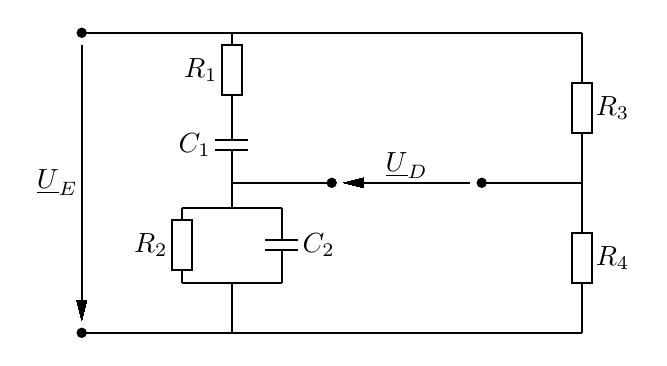
\begin{tikzpicture}[scale=2.54]%
% dpic version 2024.01.01 option -g for TikZ and PGF 1.01
\ifx\dpiclw\undefined\newdimen\dpiclw\fi
\global\def\dpicdraw{\draw[line width=\dpiclw]}
\global\def\dpicstop{;}
\dpiclw=0.8bp
\dpiclw=0.8bp
\dpicdraw (0,0)
 --(0,-0.25)\dpicstop
\dpicdraw (0,-0.5)
 --(0.05,-0.5)
 --(0.05,-0.25)
 --(-0.05,-0.25)
 --(-0.05,-0.5)
 --(0,-0.5)\dpicstop
\dpicdraw (0,-0.5)
 --(0,-0.75)\dpicstop
\draw (0.05,-0.375) node[right=-2bp]{$ R_3$};
\dpicdraw (0,-0.75)
 --(-0.5,-0.75)\dpicstop
\dpicdraw[fill=black](-0.5,-0.75) circle (0.007874in)\dpicstop
\dpicdraw[fill=black](-1.25,-0.75) circle (0.007874in)\dpicstop
\filldraw[line width=0bp](-1.09,-0.725)
 --(-1.19,-0.75)
 --(-1.09,-0.775) --cycle\dpicstop
\dpicdraw (-0.56,-0.75)
 --(-1.167094,-0.75)\dpicstop
\draw (-0.875,-0.75) node[above=-2bp]{$ \underline{U}_D$};
\dpicdraw (-1.25,-0.75)
 --(-1.75,-0.75)\dpicstop
\dpicdraw (-1.75,-0.75)
 --(-1.75,-0.5875)\dpicstop
\dpicdraw (-1.666667,-0.5875)
 --(-1.833333,-0.5875)\dpicstop
\dpicdraw (-1.666667,-0.5375)
 --(-1.833333,-0.5375)\dpicstop
\dpicdraw (-1.75,-0.5375)
 --(-1.75,-0.375)\dpicstop
\draw (-1.833333,-0.5625) node[left=-2bp]{$ C_1$};
\dpicdraw (-1.75,-0.375)
 --(-1.75,-0.3125)\dpicstop
\dpicdraw (-1.75,-0.0625)
 --(-1.8,-0.0625)
 --(-1.8,-0.3125)
 --(-1.7,-0.3125)
 --(-1.7,-0.0625)
 --(-1.75,-0.0625)\dpicstop
\dpicdraw (-1.75,-0.0625)
 --(-1.75,0)\dpicstop
\draw (-1.8,-0.1875) node[left=-2bp]{$ R_1$};
\dpicdraw (-1.75,0)
 --(0,0)\dpicstop
\dpicdraw (0,-0.75)
 --(0,-1)\dpicstop
\dpicdraw (0,-1.25)
 --(0.05,-1.25)
 --(0.05,-1)
 --(-0.05,-1)
 --(-0.05,-1.25)
 --(0,-1.25)\dpicstop
\dpicdraw (0,-1.25)
 --(0,-1.5)\dpicstop
\draw (0.05,-1.125) node[right=-2bp]{$ R_4$};
\dpicdraw (0,-1.5)
 --(-1.75,-1.5)\dpicstop
\dpicdraw (-1.75,-1.5)
 --(-1.75,-1.25)\dpicstop
\dpicdraw (-1.75,-1.25)
 --(-1.5,-1.25)\dpicstop
\dpicdraw (-1.5,-1.25)
 --(-1.5,-1.0875)\dpicstop
\dpicdraw (-1.416667,-1.0875)
 --(-1.583333,-1.0875)\dpicstop
\dpicdraw (-1.416667,-1.0375)
 --(-1.583333,-1.0375)\dpicstop
\dpicdraw (-1.5,-1.0375)
 --(-1.5,-0.875)\dpicstop
\draw (-1.416667,-1.0625) node[right=-2bp]{$ C_2$};
\dpicdraw (-1.5,-0.875)
 --(-1.75,-0.875)\dpicstop
\dpicdraw (-1.75,-1.25)
 --(-2,-1.25)\dpicstop
\dpicdraw (-2,-1.25)
 --(-2,-1.1875)\dpicstop
\dpicdraw (-2,-0.9375)
 --(-2.05,-0.9375)
 --(-2.05,-1.1875)
 --(-1.95,-1.1875)
 --(-1.95,-0.9375)
 --(-2,-0.9375)\dpicstop
\dpicdraw (-2,-0.9375)
 --(-2,-0.875)\dpicstop
\draw (-2.05,-1.0625) node[left=-2bp]{$ R_2$};
\dpicdraw (-2,-0.875)
 --(-1.75,-0.875)
 --(-1.75,-0.75)\dpicstop
\dpicdraw (-1.75,0)
 --(-2.5,0)\dpicstop
\dpicdraw[fill=black](-2.5,0) circle (0.007874in)\dpicstop
\dpicdraw[fill=black](-2.5,-1.5) circle (0.007874in)\dpicstop
\filldraw[line width=0bp](-2.525,-1.34)
 --(-2.5,-1.44)
 --(-2.475,-1.34) --cycle\dpicstop
\dpicdraw (-2.5,-0.06)
 --(-2.5,-1.417094)\dpicstop
\draw (-2.5,-0.75) node[left=-2bp]{$ \underline{U}_E$};
\dpicdraw (-2.5,-1.5)
 --(-1.75,-1.5)\dpicstop
\end{tikzpicture}%
